\documentclass[dvisvgm,multi=true]{standalone}
\usepackage{mathmlcoresvg}
\begin{document}
%<figcaption><span>Figure 14: </span>Box model for the <code>left</code>
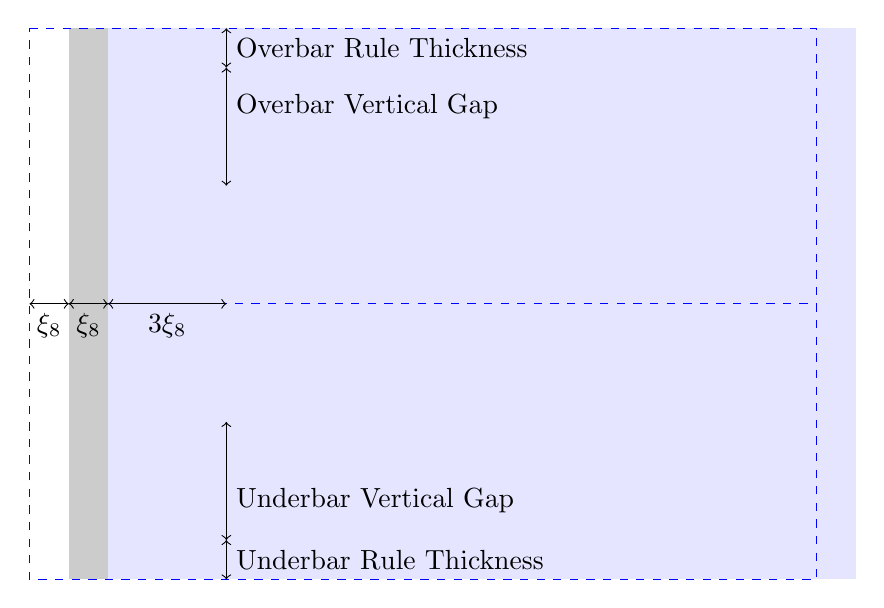
\begin{tikzpicture}[yscale=-1]

  \fill[blue!10] (0,-3.5) -- (10,-3.5) --
  (10,3.5) -- (0,3.5) -- cycle;
  \MathMLBox{2}{0}{1.5}{1}{red}

  \fill[black!20] (0,-3.5) -- (.5,-3.5) -- (.5,3.5) -- (0,3.5) -- cycle;

  \draw[dashed,blue](-.5,-3.5) -- (9.5,-3.5) -- (9.5,3.5) --
  (-.5,3.5) -- cycle (0,0) -- (9.5,0);

  \draw[<->] (2,-3) -- (2,-2.5) node[right]{Overbar Vertical Gap} -- (2,-1.5);
  \draw[<->] (2,-3) -- (2,-3.25)
    node[right]{Overbar Rule Thickness} -- (2,-3.5);

  \draw[<->] (.5,0) -- (1.25,0)node[below]{$3\xi_8$} -- (2,0);
  \draw[<->] (.5,0) -- (.25,0)node[below]{$\xi_8$} -- (0,0);
  \draw[<->] (-.5,0) -- (-.25,0)node[below]{$\xi_8$} -- (0,0);

  \draw[<->] (2,3) -- (2,2.5) node[right]{Underbar Vertical Gap} -- (2,1.5);
  \draw[<->] (2,3) -- (2,3.25)
    node[right]{Underbar Rule Thickness} -- (2,3.5);
\end{tikzpicture}

\end{document}
